% Chapter 3
\chapter{Deep Learning Models} % Main chapter title

\label{Chapter3} % For referencing the chapter elsewhere, use \ref{Chapter3} 

%----------------------------------------------------------------------------------------
In this project, deep learning models based on following deep neural networks were considered:\\
\begin{itemize}
\item \textbf{Feedforward Deep Neural Network}
\item \textbf{Deep Convolutional Neural Network}
\end{itemize}
%----------------------------------------------------------------------------------------
\section{Baseline DNN model}
A baseline deep neural network model was considered with the following architecture (See figure: \ref{fig:dnn_0}):
\begin{figure}[!htbp]
\centering
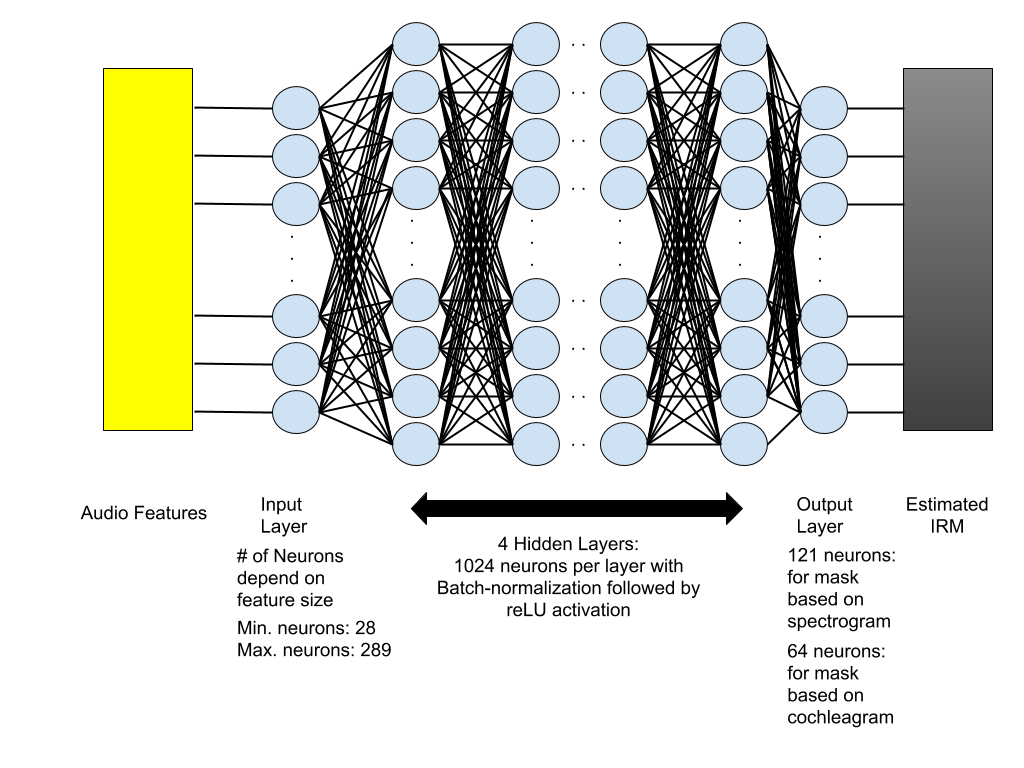
\includegraphics[width=1.2\linewidth]{dnn_0}
\caption{A Baseline feedforward deep neural network with 5 layers}
\label{fig:dnn_0}
\end{figure}
\begin{itemize}
\item \textbf{Image Input Layer}:\\
This layer accepts the feature data as a 2-D or 3-D input. The number of neurons is this layer depends on the dimension size of the features. For the different combination of features on which this DNN was trained, the minimum number of input neurons were 28 for only GFCC and MFCC features. The maximum number of neurons were 289 for a combination of Spectrogram, GFCC,GFCC Delta ,GFCC double delta, MFCC, MFCC Delta, MFCC double delta and Pitch features.
\item \textbf{Hidden Layers}:\\
Four hidden layers were used with the following properties:
\begin{itemize}
\item \textbf{Fully Connected Layer}:\\
This layer connect every neuron in one layer to every neuron in another layer \cite{wiki:cnn}.
\item \textbf{Batch Normalization}:\\
Since the activations are constantly changing during training for the intermediate layers, this slows down the training process because each layer must learn to adapt themselves to a new distribution in every training step. This problem is known as \enquote{\textit{internal covariate shift}}. Batch normalization is a method used to normalize the inputs of each layer, in order to fight the internal covariate shift problem \cite{wiki:batch}. During training time, a batch normalization layer does the following:
\begin{enumerate}
\item Calculate the mean and variance of the layers input.
\item Normalize the layer inputs using the previously calculated batch statistics.
\item Scale and shift in order to obtain the output of the layer.
\end{enumerate}
\item \textbf{reLU activation}:\\
The rectified linear unit activation function is a piecewise linear function that will output the input directly if is positive, otherwise, it will output zero \cite{wiki:relu}. This thus helps in overcoming \enquote{\textit{vanishing gradient problem}} (See 3.3) often encountered with traditional tanh or sigmoid activations. reLU activation applys the function  $$f(x)=max(0,x)$$ where \textit{x} is the output calculated post weight multiplication and bias addition at a given layer. 
\end{itemize}
\item \textbf{Output Layer}:\\
Output layer is a fully connected layer with regression operation. The number of neurons in this layer is equal to the dimension of the IRM to estimate. For a spectrogram based IRM, the number of output neurons are 121 and for a cochleagram based IRM, the number of output neurons are 64. Regression operation tries to minimize a cost function to model the feature set with respect to the IRM to estimate. The metric used for optimisation is Root Mean Square Error (RMSE) to minimize the intended cost function for modeling the training data.
\end{itemize}

\subsection{Experiments with baseline DNN}
Baseline DNN was used to identify the best feature set for speech enhancement with an emphasis on finding simpler features with improvement in the intelligibility and quality with reduced computing resource consumption. Experiments were divided into two categories based on training targets, viz \enquote{IRM based on spectrograms} and \enquote{IRM based on cochleagram}. Baseline DNN was trained for noisy mixtures at 0 SNR and -2 SNR respectively.\\

\begin{enumerate}
\item \textbf{IRM based on spectrograms}:\\
\begin{itemize}
\item \textbf{Intelligibility}:\\
STOI performance for different combination of audio features is listed in the table \ref{tab:dnn_0_stoi}. Following inferences can be made:\\ 
\begin{enumerate}
\item \textbf{Comparison between worst performing and best performing features}:\\
As evident from the table \ref{tab:dnn_0_stoi}, the gain in intelligibility from the worst performing and the best performing feature set is  \enquote{\textbf{2.5\%}} for SNR 0 and \enquote{\textbf{1.3\%}} for SNR -2.\\ 
\item \textbf{Comparison of intelligibility with noisy audios}:\\
On comparing with the intelligibilty scores of the original noisy mixture for the best performing feature set (See table: \ref{tab:stoi_mix}) the gain in intelligibility scores for SNR 0 is \enquote{\textbf{10.9\%}} and for SNR -2 is \enquote{\textbf{14.9\%}}.\\
\end{enumerate}
\begin{table}[!htbp]
\centering
\begin{tabular}{ |p{12cm}|p{1.7cm}|p{1.7cm}|  }
\hline
\textbf{Features} & \multicolumn{2}{|c|}{\textbf{STOI}} \\
\hline
\cellcolor{black} & SNR 0 & SNR -2 \\
\hline
Spectrogram & 0.81	& 0.76\\
\hline
Spectrogram, MFCC, MFCC Delta, MFCC delta delta & 0.80	& 0.77\\
\hline
Spectrogram, Pitch &	0.79 & 0.76\\
\hline
Spectrogram, GFCC, GFCC Delta, GFCC delta delta & 0.80	& 0.77\\
\hline
Spectrogram, GFCC, GFCC Delta, GFCC delta delta, MFCC, MFCC Delta, MFCC delta delta &	0.80 & 0.77\\
\hline
GFCC, MFCC & 0.79 & 0.76\\
\hline
Spectrogram, GFCC, MFCC & 0.80 & 0.77\\
\hline
\rowcolor[HTML]{ADD8E6}GFCC, GFCC Delta, GFCC delta delta & 0.81 & 0.77\\
\hline
GFCC, GFCC Delta, GFCC delta delta, MFCC, MFCC delta, MFCC delta delta &	0.81 & 0.77\\
\hline
Spectrogram, GFCC, GFCC delta, GFCC delta delta, MFCC, MFCC delta, MFCC delta delta, Pitch & 0.79 & 0.76\\
\hline
MFCC, MFCC delta, MFCC delta delta & 0.80 & 0.77\\
\hline
\end{tabular}
\caption{STOI performance: Baseline, IRM based on spectrogram}
\label{tab:dnn_0_stoi}
\end{table}

\item \textbf{Quality}:\\
PESQ performance for different combination of audio features is listed in the table \ref{tab:dnn_0_pesq}.Following inferences can be made:\\
\begin{enumerate}
\item \textbf{Comparison of quality gain from worst to best performing feature set}:\\
The quality gain from the worst performing feature set to the best performing feature set is \enquote{\textbf{9.9\%}} for \textbf{PESQMOS} and \enquote{\textbf{11.5\%}} for \textbf{MOSLQO}  for SNR 0. For SNR -2 the gain in quality is \enquote{\textbf{6.6\%}} for \textbf{PESQMOS} and \enquote{\textbf{8.8\%}} for \textbf{MOSLQO} respectively.
\item \textbf{Comparison of quality gain from noisy mixtures}:\\
It's also important to compare the gain in quality in estimated speech signal as compared to the quality scores of the noisy mixture which  has been tabulated in \ref{tab:pesq_mix} for  the best performing feature set, for SNR 0 and -2 respectively. Hence, comparing both tables gives us a gain in quality of \enquote{\textbf{10.5\%}} for \textbf{PESQMOS} and \enquote{\textbf{10.9\%}} for \textbf{MOSLQO} at SNR 0 and the gain in quality of \enquote{\textbf{9.8\%}} for \textbf{PESQMOS} and \enquote{\textbf{11.3\%}} for \textbf{MOSLQO} at SNR -2 respectively.
\end{enumerate} 
\begin{table}[!htbp]
\centering
\begin{tabular}{ |p{8cm}|p{1.7cm}|p{1.7cm}|p{1.7cm}|p{1.7cm}|  }
\hline
\textbf{Features} & \multicolumn{4}{|c|}{\textbf{PESQ}}\\
\hline
\cellcolor{black} & \multicolumn{2}{|c|}{SNR 0} & \multicolumn{2}{|c|}{SNR -2}\\
\hline
\cellcolor{black} & PESQMOS & MOSLQO & PESQMOS & MOSLQO\\
\hline
Spectrogram	& 2.11	& 1.82	& 2.10	& 1.81\\
\hline
Spectrogram,MFCC,MFCC delta,MFCC delta delta	& 2.31	& 2.03	& 2.21	& 1.93\\
\hline
Spectrogram,Pitch	& 2.23	& 1.95	& 2.18	& 1.93\\
\hline
\cellcolor{yellow}Spectrogram,GFCC,GFCC delta,GFCC delta delta	& 2.29	& 1.99	& \cellcolor{yellow}2.24	& \cellcolor{yellow}1.97\\
\hline
Spectrogram,GFCC,GFCC delta,GFCC delta delta MFCC,MFCC delta,MFCC delta delta	& 2.30	& 2.02	& 2.19	& 1.92\\
\hline
GFCC,MFCC	& 2.26	& 1.96	& 2.16	& 1.88\\
\hline
Spectrogram,GFCC,MFCC	& 2.29	& 2.00	& 2.22	& 1.95\\
\hline
\cellcolor[HTML]{ADD8E6}GFCC,GFCC delta,GFCC delta delta	& \cellcolor[HTML]{ADD8E6}2.32	& \cellcolor[HTML]{ADD8E6}2.03	& 2.20	& 1.92\\
\hline
GFCC,GFCC delta,GFCC delta delta MFCC,MFCC delta,MFCC delta delta	& 2.28	& 1.99	& 2.19	& 1.90\\
\hline
Spectrogram,GFCC,GFCC delta,GFCC delta delta MFCC,MFCC delta,MFCC delta delta,Pitch	& 2.19	& 1.90	& 2.16	& 1.87\\
\hline
MFCC,MFCC delta,MFCC delta delta	& 2.26	& 1.98	& 2.13	& 1.85\\
\hline
\end{tabular}
\caption{PESQ performance: Baseline, IRM based on spectrogram}
\label{tab:dnn_0_pesq}
\end{table}

\begin{table}[!htbp]
\centering
\begin{tabular}{ |p{8cm}|p{1.7cm}|p{1.7cm}|p{1.7cm}|p{1.7cm}|  }
\hline
\textbf{Features} & \multicolumn{4}{|c|}{\textbf{PESQ}}\\
\hline
\cellcolor{black} & \multicolumn{2}{|c|}{SNR 0} & \multicolumn{2}{|c|}{SNR -2}\\
\hline
Noise mixed speech samples & 2.10 & 1.83 & 2.04 & 1.73\\
\hline
\end{tabular}
\caption{PESQ values for noisy mixture}
\label{tab:pesq_mix}
\end{table}
 
\end{itemize}
\item \textbf{IRM based on cochleagrams}:\\
\begin{itemize}
\item \textbf{Intelligibility}:\\
STOI performance for different combination of audio features is listed in the table \ref{tab:dnn_0_stoi_1}. Following inferences can be made.\\
\begin{enumerate}
\item \textbf{Comparison with the IRM based on Spectrogram}:\\
As evident from the table \ref{tab:dnn_0_stoi_1}, the gain in intelligibility score for the best performing feature sets is \enquote{\textbf{1.2\%}} when compared to the best performing feature set for the IRM based on spectrogram for SNR 0 and for SNR -2 the intelligibility scores are the same for both the cases.
\item \textbf{Comparison from the worst to best performing feature set}:\\
The gain in intelligibility score from worst performing feature set to the best performing feature set is by \enquote{\textbf{6.5\%}} for SNR 0 and \enquote{\textbf{6.9\%}} for SNR -2.\\ 
\item \textbf{Gain in intelligibility from noisy mixtures}:\\
For the best perfroming feature set, when compared to the original noisy mixture's intelligibility (see table: \ref{tab:stoi_mix}), the gain is \enquote{\textbf{12.3\%}} for SNR 0 and for SNR -2, the gain in intelligibility is \enquote{\textbf{14.9\%}}.\\ 
\end{enumerate}
Hence, it highlights a better performance than the IRM based on spectrograms for the intelligibility gains.

\item \textbf{Quality}:\\
PESQ performance for different combination of audio features is listed in the table \ref{tab:dnn_0_pesq_2}. Following observations can be made:\\ 
\begin{enumerate}
\item \textbf{Comparison with IRM based on spectrogram}:\\
As it's evident from the table \ref{tab:dnn_0_pesq_2}, the quality scores are better as compared to IRM based on spectrogram for the best performing feature sets in the both cases by around 2.1\% for 0 SNR and by around 3.1\% for -2 SNR considering PESQMOS as quality metric for the best performing feature set. 
\item \textbf{Comparison of quality gain from worst to best performing feature set}:\\
Quality gain from the worst performing feature set to the best performing feature set is by \enquote{\textbf{9.7\%}} for \textbf{PESQMOS} and \enquote{\textbf{11.9\%}} for \textbf{MOSLQO} at SNR 0. At SNR -2 the gain in quality is \enquote{\textbf{13.8\%}} for \textbf{PESQMOS} and  \enquote{\textbf{14.3\%}} for \textbf{MOSLQO}.
\item \textbf{Comparison with the quality of noisy mixtures}:\\
On comparing for quality gain from the noisy mixtures for the best performing feature set as tabulated in the table \ref{tab:pesq_mix}, there is a gain of \enquote{\textbf{12.8\%}} for \textbf{PESQMOS} and \enquote{\textbf{13.1\%}} for \textbf{MOSLQO} at SNR 0 and the gain in quality of \enquote{\textbf{13.2\%}} for \textbf{PESQMOS} and \enquote{\textbf{15.6\%}} for \textbf{MOSLQO} at SNR -2 respectively.
\end{enumerate}
This highlights the importance of \enquote{\textbf{Cochleagram}} as  training data for low SNR scenarios and also highlight the overall improvement in quality when using cochleagram based masks as compared to spectrogram based masks during training.
\end{itemize}
\end{enumerate}

\begin{table}[!htbp]
\centering
\begin{tabular}{ |p{12cm}|p{1.7cm}|p{1.7cm}|  }
\hline
\textbf{Features} & \multicolumn{2}{|c|}{\textbf{STOI}} \\
\hline
\cellcolor{black} & SNR 0 & SNR -2 \\
\hline
\rowcolor[HTML]{ADD8E6}Cochleagram	& 0.82	& 0.77\\
\hline
GFCC,GFCC delta,GFCC delta delta	& 0.78	& 0.73\\
\hline
GFCC,GFCC delta,GFCC delta delta MFCC,MFCC delta,MFCC delta delta	& 0.77	& 0.74\\
\hline
MFCC,MFCC delta,MFCC delta delta	& 0.78	& 0.75\\
\hline
GFCC,MFCC	& 0.78	& 0.74\\
\hline
\end{tabular}
\caption{STOI performance: Baseline, IRM based on cochleagram}
\label{tab:dnn_0_stoi_1}
\end{table}

\begin{table}[!htbp]
\centering
\begin{tabular}{ |p{8cm}|p{1.7cm}|p{1.7cm}|p{1.7cm}|p{1.7cm}|  }
\hline
\textbf{Features} & \multicolumn{4}{|c|}{\textbf{PESQ}}\\
\hline
\cellcolor{black} & \multicolumn{2}{|c|}{SNR 0} & \multicolumn{2}{|c|}{SNR -2}\\
\hline
\cellcolor{black} & PESQMOS & MOSLQO & PESQMOS & MOSLQO\\
\hline
\cellcolor[HTML]{ADD8E6}Cochleagram	& \cellcolor[HTML]{ADD8E6}2.37	& \cellcolor[HTML]{ADD8E6}2.07	& \cellcolor{yellow}2.31	& \cellcolor{yellow}2.00\\
\hline
GFCC,GFCC delta,GFCC delta delta	& 2.23	& 1.92	& 2.05	& 1.75\\
\hline
GFCC,GFCC delta,GFCC delta delta MFCC,MFCC delta,MFCC delta delta	& 2.21	& 1.91	& 2.09	& 1.80\\
\hline
MFCC,MFCC delta,MFCC delta delta	& 2.16	& 1.85	& 2.09	& 1.82\\
\hline
GFCC,MFCC	& 2.27	& 1.96	& 2.06	& 1.77\\
\hline
\end{tabular}
\caption{PESQ performance: Baseline, IRM based on cochleagram}
\label{tab:dnn_0_pesq_2}
\end{table}


\begin{table}[!htbp]
\centering
\begin{tabular}{ |p{12cm}|p{1.7cm}|p{1.7cm}|  }
\hline
\textbf{Features} & \multicolumn{2}{|c|}{\textbf{STOI}} \\
\hline
\cellcolor{black} & SNR 0 & SNR -2 \\
\hline
Noise Mixed Speech Samples	& 0.73	& 0.67\\
\hline
\end{tabular}
\caption{STOI values for Noise Mixed speech samples}
\label{tab:stoi_mix}
\end{table}
%--------------------------------------------------------------------------------------
\section{DNN model based on biased sigmoid activation}
Another deep neural network model was considered with the following architecture (See figure: \ref{fig:dnn_1}):
\begin{itemize}
\item \textbf{Image Input Layer}:\\
This layer accepts the feature data as a 2-D or 3-D input. The number of neurons is this layer depends on the dimension size of the features just as with the baseline model.
\item \textbf{Hidden Layers}:\\
Four hidden layers were used with the following properties:
\begin{itemize}
\item \textbf{Fully Connected Layer}:\\
This layer connect every neuron in one layer to every neuron in another layer.
\item \textbf{Biased Sigmoid Layer}:\\
This layer is an alteration on a sigmoid layer which uses a sigmoid activation function (See figure: \ref{fig:sigmoid}) to overcome \enquote{\textit{vanishing gradient problem}}. The number of neurons in these layers are twice the number of neurons in the input layer. Sigmoid function, squishes a large input space into a small input space between 0 and 1. Therefore, a large change in the input of the sigmoid function will cause a small change in the output. Hence, the derivative becomes small. This causes the neural network to have a reduced learning with the gradients not able to reach the optimization points over time. The biased sigmoid activation layer overcomes this problem by enforcing the sigmoid function to operate on it's linear part where the derivative of the function is significantly better than the case when the sigmoid function operates closer to the region of 0 and 1. Hence, the biased sigmoid layer is able to overcome the \enquote{\textit{Vanishing Gradient Problem}}. The purpose of using this layer is to compare it's performance with the reLU activation used in the baseline DNN as discussed in the previous section. 
\item \textbf{Batch Normalization}:\\
As discussed in the previous section, this layer helps in overcoming\enquote{\textit{internal covariate shift}}. It does so by normalizing the inputs of each layer.
\item \textbf{Dropout Layer}:\\
This layer works on a tunable parameter called the \enquote{\textit{Dropout Probability}}. During the training phase, the proportion of neurons as defined by the parameter \enquote{\textit{Dropout Probability}} on a particular layer are deactivated. This improve generalization because it forces a layer to learn with different neurons the same "concept". Hence, this is used to prevent overfitting of the training data, where a learning machine has an ability to model the training data but performs poorly on the testing data. During the prediction phase however, the dropout is deactivated.
\end{itemize}
\begin{figure}[!htbp]
\centering
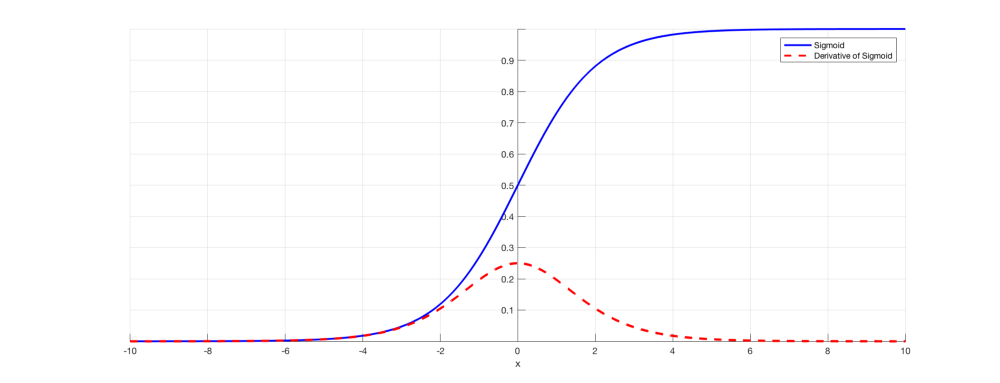
\includegraphics[width=1.1\linewidth]{sigmoid}
\caption{Sigmoid activation function.}
\label{fig:sigmoid}
\end{figure}
\item \textbf{Output Layer}:\\
Output layer is a fully connected layer with biased sigmoid activation and  regression operation. The number of neurons in this layer is equal to the dimension of the IRM to estimate. For a spectrogram based IRM, the number of output neurons are 121 and for a cochleagram based IRM, the number of output neurons are 64. Biased sigmoid layer tries to prevent \enquote{\textit{Vanishing Gradient Problem}} followed by a regression operation, which tries to minimize a cost function to model the feature set with respect to the IRM to estimate by using RMSE as an optimization metric.
\end{itemize}
\begin{figure}[!htbp]
\centering
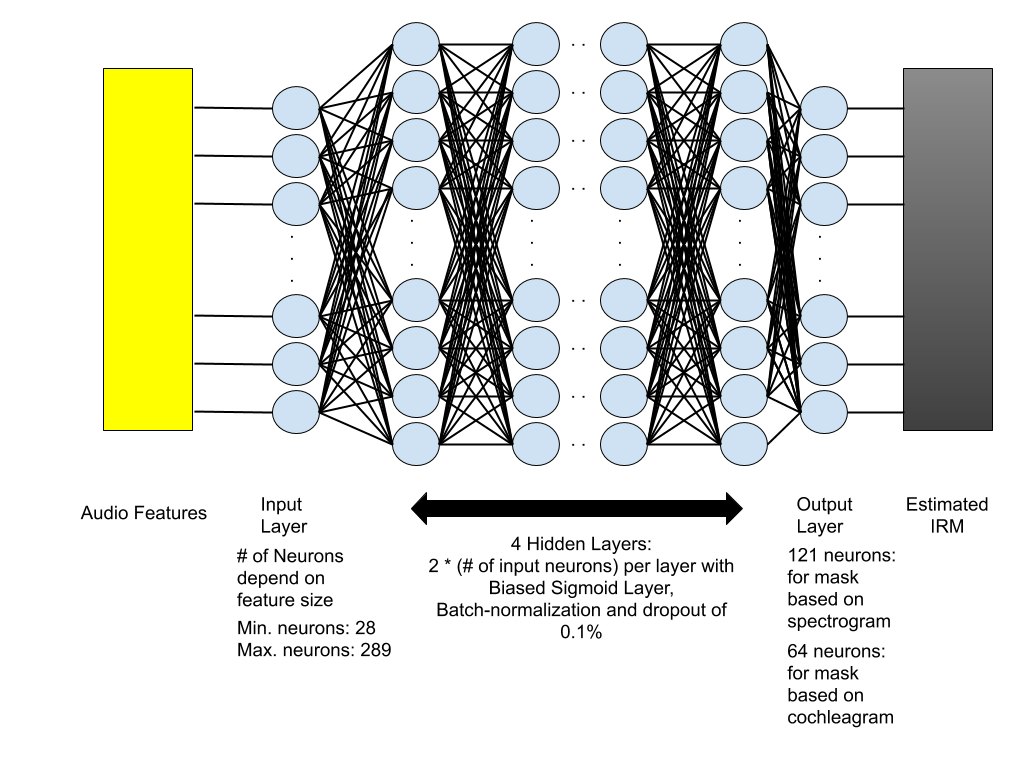
\includegraphics[width=1.2\linewidth]{dnn_1}
\caption{A feedforward deep neural network with 5 layers and biased sigmoid activation}
\label{fig:dnn_1}
\end{figure}

\subsection{Experiments with the DNN using biased activation}
Using the results from the baseline DNN, experiments were conducted using the best performing feature sets with the baseline DNN. Similar to the baseline DNN, experiments were divided into two categories based on training targets, viz “IRM based on spectrograms” and “IRM based on cochleagram”. Training was done for noisy mixtures at 0 SNR and -2 SNR respectively.
\begin{enumerate}
\item \textbf{IRM based on Spectrogram}
\begin{itemize}
\item \textbf{Intelligibility}:\\
STOI performance for different combination of audio features is listed in
the table \ref{tab:dnn_1_stoi_1}. Following observations can be made:\\
\begin{enumerate}
\item \textbf{Comparison with the baseline DNN}:\\
As it's evident from the table \ref{tab:dnn_1_stoi_1}, there is no significant improvement in the intelligiblity scores as compared to the baseline DNN's performance tabulated in the table \ref{tab:dnn_0_stoi_1}. Infact for the best performning feature set, the intelligibilty score is reduced by \enquote{\textbf{1.25\%}} for SNR 0. Although the intelligibility for SNR -2 as compared to the baseline DNN is the same for the same feature set.
\item \textbf{Comparison of intelligibility gain from worst to the best performing features}:\\
The improvement in intelligibility for the feature sets used for this experiment from the worst performing to the best performing set is by \enquote{\textbf{2.5\%}} for SNR 0 and for SNR -2, the improvement is \enquote{\textbf{4\%}}.
\item \textbf{Comparison with the noisy mixtures}:
The intelligibility gains as compared to the noisy mixtures (see table: \ref{tab:stoi_mix}) is \enquote{\textbf{9.6\%}} for SNR 0 and for SNR -2 the gain is of \enquote{\textbf{14.9\%}}.
\end{enumerate}
The best performing feature set in this case was still found out to be \enquote{\textbf{GFCC, GFCC delta, GFCC delta delta}} for both SNR 0 and SNR -2 which is similar to the performance of this feature set with the baseline DNN for SNR 0 whereas in the case of the baseline DNN for -2 SNR, the best feature set was \enquote{\textbf{Spectrogram, GFCC, GFCC delta, GFCC delta delta}}. This reflects a strong correlation of GFCC related feature set with the IRM based on spectrogram. However, overall the intelligibilty performance shows no significant improvement as compared to the baseline DNN for this deep learning model.

\begin{table}[!htbp]
\centering
\begin{tabular}{ |p{12cm}|p{1.7cm}|p{1.7cm}|  }
\hline
\textbf{Features} & \multicolumn{2}{|c|}{\textbf{STOI}} \\
\hline
\cellcolor{black} & SNR 0 & SNR -2\\
\hline
Spectrogram	& 0.79	& 0.76\\
\hline
Spectrogram,GFCC,GFCC delta,GFCC delta delta	& 0.80	& 0.76\\
\hline
Spectrogram,GFCC,MFCC	& 0.78	& 0.77\\
\hline
\rowcolor[HTML]{ADD8E6}GFCC,GFCC delta,GFCC delta delta	& 0.80	& 0.77\\
\hline
GFCC,GFCC delta,GFCC delta delta MFCC,MFCC delta,MFCC delta delta	& 0.79	& 0.74\\
\hline
\end{tabular}
\caption{STOI performance: DNN2, IRM based on spectrogram}
\label{tab:dnn_1_stoi_1}
\end{table}

\item \textbf{Quality}:\\
PESQ performance for different combination of audio features is listed in
the table \ref{tab:dnn_1_pesq_1}. Following inferences can be made:\\
\begin{enumerate}
\item \textbf{Comparison with the baseline DNN}:\\
From the table \ref{tab:dnn_1_pesq_1}, and comparing the PESQ scores with the baseline DNN documented in the table \ref{tab:dnn_0_pesq}, the scores show deterioration of the quality. The best performing feature set \enquote{\textit{Spectrogram,GFCC,GFCC delta,GFCC delta delta}}, shows detereoration of \enquote{\textbf{0.8\%}} for \textbf{PESQMOS} score and detereoration of \enquote{\textbf{0.9\%}} for the \textbf{MOSLQO} score when compared to the performance of the best performing feature set found for the baseline DNN at SNR 0. For SNR -2, the best performing feature set \enquote{\textbf{GFCC, GFCC delta, GFCC delta delta}} showed the detereoration of \enquote{\textbf{1.8\%}} for the \textbf{PESQMOS} score, and the \textbf{MOSLQO} scores were the same at \enquote{1.97}.
\item \textbf{Comparison of quality gain from worst to the best performing feature}:\\
For this experiment the gain of quality from the worst performing feature set to the best performing feature set was of \enquote{\textbf{8.4\%}} for \textbf{PESQMOS} and \enquote{\textbf{5.2\%}} for \textbf{MOSLQO} at SNR 0. At SNR -2, the gain in quality from the worst to the best performing feature set was of \enquote{\textbf{10\%}} for \textbf{PESQMOS} and \enquote{\textbf{8.2\%}} for \textbf{MOSLQO}.
\item \textbf{Comparison with the noisy mixture}:\\
On comparing the quality gain for the best performing feature set in this experiment from the noisy mixture as documented in the table \ref{tab:dnn_1_pesq_1} the gain was \enquote{\textbf{9.5\%}} for \textbf{PESQMOS} and \enquote{\textbf{9.8\%}} for \textbf{MOSLQO} at SNR 0. At SNR -2, the gain was \enquote{\textbf{7.8\%}} for \textbf{PESQMOS} and \enquote{\textbf{11.3\%}} for \textbf{MOSLQO}.
\end{enumerate}
Overall, it can be said that there is no significant improvement when comapred to the quality gain performance of the baseline DNN for this deep learning model.
\begin{table}[!htbp]
\centering
\begin{tabular}{ |p{8cm}|p{1.7cm}|p{1.7cm}|p{1.7cm}|p{1.7cm}|  }
\hline
\textbf{Features} & \multicolumn{4}{|c|}{\textbf{PESQ}}\\
\hline
\cellcolor{black} & \multicolumn{2}{|c|}{SNR 0} & \multicolumn{2}{|c|}{SNR -2}\\
\hline
\cellcolor{black} & PESQMOS & MOSLQO & PESQMOS & MOSLQO\\
\hline
Spectrogram	& 2.21	& 1.91	& 2.17	& 1.90\\
\hline
\cellcolor[HTML]{ADD8E6}Spectrogram,GFCC,GFCC delta,GFCC delta delta	& \cellcolor[HTML]{ADD8E6}2.30	& \cellcolor[HTML]{ADD8E6}2.01	& 2.12	& 1.82\\
\hline
Spectrogram,GFCC,MFCC	& 2.22	& 1.98	& 2.00	& 1.93\\
\hline
\cellcolor{yellow}GFCC,GFCC delta,GFCC delta delta	& 2.28	& 1.99	& \cellcolor{yellow}2.20	& \cellcolor{yellow}1.97\\
\hline
GFCC,GFCC delta,GFCC delta delta MFCC,MFCC delta,MFCC delta delta	& 2.12	& 1.97	& 2.00	& 1.89\\
\hline
\end{tabular}
\caption{PESQ performance: DNN2, IRM based on spectrogram}
\label{tab:dnn_1_pesq_1}
\end{table}
\end{itemize}

\item \textbf{IRM based on Cochleagram}
\begin{itemize}
\item \textbf{Intelligibility}
STOI performance for different combination of audio features is listed in the table \ref{tab:dnn_1_stoi_2}. Following observations can be made:\\
\begin{enumerate}
\item \textbf{Comparison with the baseline DNN}:\\
From the table \ref{tab:dnn_1_stoi_2}, shows a detereoration in the intelligibility score as comapred to the baseline DNN's performance by \enquote{\textbf{2.5\%}} for SNR 0 and for SNR -2, by \enquote{\textbf{1.3\%}} for the best performing feature set.
\item \textbf{Comparison from the worst and the best performing feature set}:\\
Since the intelligibility performance was poor with the feature sets in the previous experiment with IRM based on spectrogram, this experiment was confined to the best performing set of \enquote{\textit{GFCC, GFCC delta, GFCC delta delta}} and \enquote{\textit{Cochleagram}}. Within this experiment, the intelligibility gain from worst performing feature set to the best performing feature set is \enquote{\textbf{3.9\%}} for SNR 0 and for SNR -2, the gain was \enquote{\textbf{5.5\%}}.
\item \textbf{Comparison with the noisy mixtures}:\\
On comparing with the intelligibility of the noisy mixtures (see table: \ref{tab:stoi_mix}), the gain was found out to be \enquote{\textbf{9.6\%}} at 0 SNR and at \enquote{\textbf{13.4\%}} -2 SNR for \enquote{\textit{Cochleagram}} as the better performing feature set in the previous case.
\end{enumerate}
This shows an improvement in intelligibility scores when using IRM based on cochleagram as training target compared to the IRM based on spectrogram which is as per the trend with the baseline DNN as well. However, compared to intelligibility gains provided by the baseline DNN, this deep learning model shows no significant improvement.
\begin{table}[!htbp]
\centering
\begin{tabular}{ |p{12cm}|p{1.7cm}|p{1.7cm}|  }
\hline
\textbf{Features} & \multicolumn{2}{|c|}{\textbf{STOI}} \\
\hline
\cellcolor{black} & SNR 0 & SNR -2\\
\hline
\rowcolor[HTML]{ADD8E6}Cochleagram	& 0.80	& 0.76\\
\hline
GFCC, GFCC delta, GFCC delta delta & 0.77	& 0.72\\
\hline
\end{tabular}
\caption{STOI performance: DNN2, IRM based on cochleagram}
\label{tab:dnn_1_stoi_2}
\end{table}

\item \textbf{Quality}
PESQ performance for the different combination of audio features is listed in the table \ref{tab:dnn_1_pesq_2}. Following inferences can be made:\\
\begin{enumerate}
\item \textbf{Comparison with the baseline DNN}:\\
On comparing the tabulated data from the table \ref{tab:dnn_1_pesq_2}, with the baseline DNN's performance in the table \ref{tab:dnn_0_pesq_2}, for the best performing feature set, there is detereoration in quality by \enquote{\textbf{1.7\%}} for \textbf{PESQMOS} and \enquote{\textbf{0.9\%}} for \textbf{MOSLQO} for SNR 0. For SNR -2, the detereoration is by \enquote{\textbf{1.7\%}} for \textbf{PESQMOS} and \enquote{\textbf{1\%}} for \textbf{MOSLQO}.
\item \textbf{Comparison from the worst to best performing feature set}:\\
Within this experiment the gain in quality from the worst perfroming feature set to the best performing feature set was found out to be \enquote{\textbf{8.1\%}} for \textbf{PESQMOS} and \enquote{\textbf{9.9\%}} for \textbf{MOSLQO} for SNR 0. For SNR -2, the detereoration is by \enquote{\textbf{11.8\%}} for \textbf{PESQMOS} and \enquote{\textbf{13.1\%}} for \textbf{MOSLQO}.
\item \textbf{Comparison with the noisy mixture}:\\
On comapring with the quality of noisy mixtures as tabulated in the table \ref{tab:pesq_mix}, the gain in quality was found out to be \enquote{\textbf{11.2\%}} for \textbf{PESQMOS} and \enquote{\textbf{12.9\%}} for \textbf{MOSLQO} for SNR 0. For SNR -2, the detereoration is by \enquote{\textbf{13.5\%}} for \textbf{PESQMOS} and \enquote{\textbf{13.8\%}} for \textbf{MOSLQO} respectively.
\end{enumerate}
Overall, this too shows no significant improvement in quality gains as comaperd with the gains provided by the baseline DNN.
\begin{table}[!htbp]
\centering
\begin{tabular}{ |p{8cm}|p{1.7cm}|p{1.7cm}|p{1.7cm}|p{1.7cm}|  }
\hline
\textbf{Features} & \multicolumn{4}{|c|}{\textbf{PESQ}}\\
\hline
\cellcolor{black} & \multicolumn{2}{|c|}{SNR 0} & \multicolumn{2}{|c|}{SNR -2}\\
\hline
\cellcolor{black} & PESQMOS & MOSLQO & PESQMOS & MOSLQO\\
\hline
\cellcolor[HTML]{ADD8E6}Cochleagram	& \cellcolor[HTML]{ADD8E6}2.39	& \cellcolor[HTML]{ADD8E6}2.10	& \cellcolor{yellow}2.27	& \cellcolor{yellow}1.98\\
\hline
GFCC, GFCC delta, GFCC delta delta & 2.21	& 1.91	& 2.03	& 1.75\\
\hline
\end{tabular}
\caption{PESQ performance: DNN2,IRM based on cochleagram}
\label{tab:dnn_1_pesq_2}
\end{table}
\end{itemize}
\end{enumerate}
%--------------------------------------------------------------------------------------
\section{Deep Learning Model based on CNN}
A deep learning model based on Convolutional Neural Networks (See figure: \ref{fig:cnn}) places less demand on the features as they have an ability to find patterns in the training data by themselves. Exploiting this nature, the experiments with this learning model were confined to the two prominent visual representations of the audio signals namely, Spectrograms and Cochleagrams. The architecture of the considered deep CNN was as following:
\begin{figure}[!htbp]
\centering
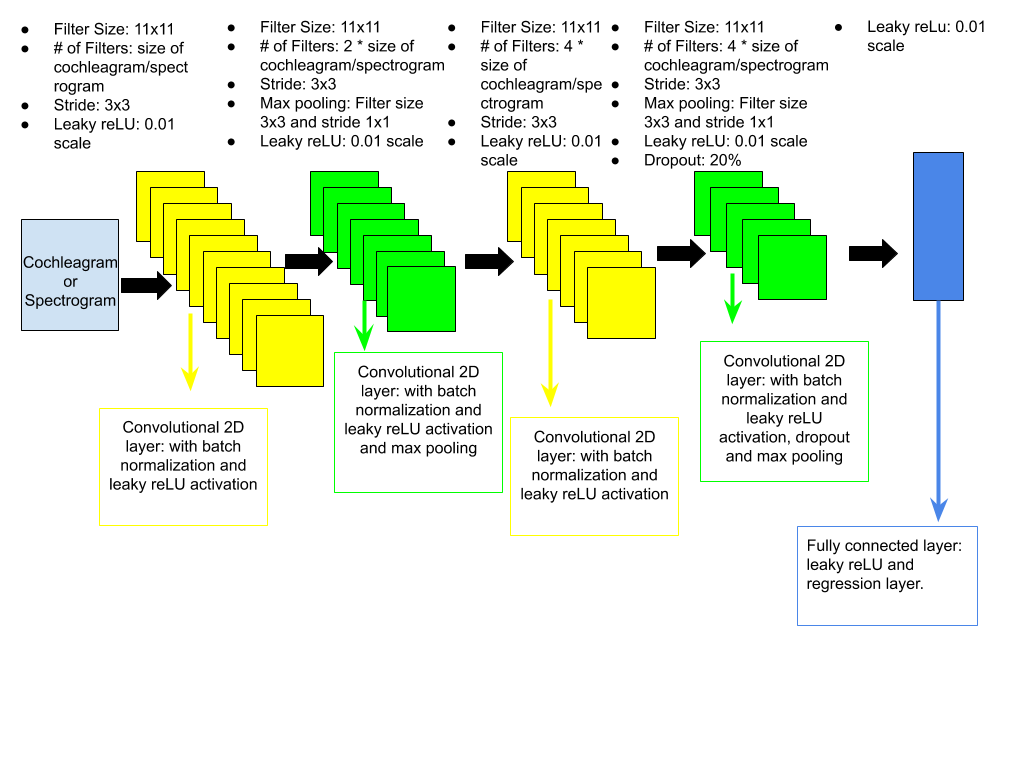
\includegraphics[width=1.2\linewidth]{cnn}
\caption{A CNN with 4 2-D Convolutional Layers and 2 downsampling 2-D Maxpooling Layers}
\label{fig:cnn}
\end{figure}
\begin{itemize}
\item \textbf{Image Input Layer}:\\
As described in the previous sections, this layer accepts the feature data as a 2-D or 3-D input. The number of neurons is this layer depends on the dimension size of the features. For cochleagram based training data, the number of input neurons are 64 and for spectrogram based training data, the number of input neurons are 121.

\item \textbf{Hidden Layers}:\\
Hidden layers in considered deep CNN were combination of \textbf{four} convolution2dLayer(s) with a downsampling by maxPooling2dLayer(s) after second and fourth convolution2dLayer respectively. The hidden layers had the following properties:
\begin{itemize}
\item \textbf{Convolution2dLayer}:\\
This is a 2-D convolutional layer which applies sliding convolutional filters to the input. The layer convolves the input by moving the filters along the input vertically and horizontally and computing the dot product of the weights and the input, and then adding a bias term. The convolutional \textbf{filter's kernel size} was kept at \textbf{11x11} and the \textbf{number of convolutional filters} were kept the \textbf{same as feature size i.e 64/121} for the \textbf{first} convolution2dLayer, \textbf{2x(feature size i.e 64/121)} for the \textbf{second} convolution2dLayer and \textbf{4x(feature size i.e 64/121)} for the \textbf{remaining two} convolution2dLayer(s).
\item \textbf{Batch Normalization}:
As discussed in the previous sections, this layer helps in overcoming “internal covariate shift” problem. It does so by normalizing the inputs of each layer.
\item \textbf{Leaky reLU activation}:\\
Using reLU activation often encounters a \enquote{\textit{Dying ReLU problem}} i.e. when inputs approach zero, or are negative, the gradient of the function becomes zero, the network cannot learn these inputs. Leaky reLU prevents the dying ReLU problem by making a slight variation on ReLU by having a small positive slope in the negative area (See figure: \ref{fig:leaky_relu}), so it does enable the network to learn, even for negative input values. The leaky reLU uses the following activation function to achieve this using the scale value of 0.01 as was considered in our implementation:
\[
  f(y) =
  \begin{cases}
    	y & \text{if $y>0$} \\
        0.01y & \text{otherwise} \\
  \end{cases}
\]
\begin{figure}[!htbp]
\centering
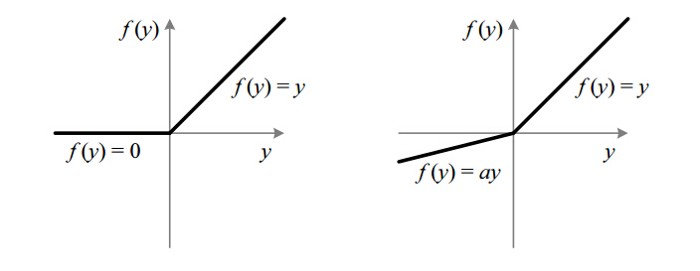
\includegraphics[width=1\linewidth]{leaky_relu}
\caption{Leaky reLU as compared to reLU}
\label{fig:leaky_relu}
\end{figure}
\item \textbf{MaxPooling2dLayer}:\\
This layer performs the down-sampling by dividing the input into rectangular pooling regions, and computing the maximum of each region. In our implementation, the max pooling filter of size \textbf{3x3} was considered.
\end{itemize}
\item \textbf{Output Layer}:\\
Output layer is a fully connected layer with leaky reLU activation and regression operation. For a spectrogram based IRM, the number of output neurons are 121 and for a cochleagram based IRM, the number of output neurons are 64. Regression operation tries to minimize a cost function to model the spectrogram/cochleagram with respect to the IRM to estimate. The metric used for optimisation is RMSE to minimize the intended cost function for modeling the training data.
\end{itemize}
\subsection{Experiments with the deep CNN}
The CNN was trained using spectrogram and cochleagram as training data. The intended training target for spectrogram was IRM based on spectrogram and for cochleagram was IRM based on cochleagram respectively. The performance analysis are as below:
\begin{itemize}
\item \textbf{Intelligibility}:\\
The STOI values for 0 and -2 SNR are documented in the table \ref{tab:cnn_stoi}. As per the information from this table following observations can be made:
\begin{enumerate}
\item \textbf{Comparison with the baseline DNN}:\\
For the best performing feature set, the gain in intelligibilty has been observed for CNN based learning model to be of \textbf{4.8\%} and \textbf{3.9\%} for 0 and -2 SNR respectively.
\item \textbf{Comparison between worst and best performing training data}:\\
The gain in intelligibility from the worst to the best performing training data is \textbf{8.8\%} and \textbf{5.3\%} for 0 and -2 SNR respectively. Since, only spectrogram and cochleagram was used as the training data, this is a comparison of intelligibility gain from spectrogram to cochleagram as training data.
\item \textbf{Intelligibility gain from the noisy mixture audios}:\\
The gain in intelligibility when considering the original noisy mixture (See table: \ref{tab:stoi_mix}) for the best performing training data was found out to be \textbf{17.8\%} and \textbf{19.4\%} for 0 and -2 SNR respectively.
\end{enumerate}
This points out that for cochleagram based training data and IRM based on the cochleagram the intelligibility gain is the best when compared to the previous learning models.
\begin{table}[!htbp]
\centering
\begin{tabular}{ |p{12cm}|p{1.7cm}|p{1.7cm}|  }
\hline
\textbf{Features} & \multicolumn{2}{|c|}{\textbf{STOI}} \\
\hline
\cellcolor{black} & SNR 0 & SNR -2\\
\hline
\rowcolor[HTML]{ADD8E6}Cochleagram	& 0.86	& 0.80\\
\hline
Spectrogram	& 0.79	& 0.76\\
\hline
\end{tabular}
\caption{STOI performance: CNN}
\label{tab:cnn_stoi}
\end{table}
\item \textbf{Quality}:\\
The PESQ values for 0 and -2 SNR are documented in the table \ref{tab:cnn_pesq}. As per the information from this table following observations can be made:
\begin{enumerate}
\item \textbf{Comparison with the baseline DNN}:\\
On comparing the tabulated data from the table \ref{tab:cnn_pesq}, with the baseline DNN's performance in the table \ref{tab:dnn_0_pesq_2}, for the best performing feature set, there is gain in quality by \enquote{\textbf{2.1\%}} for \textbf{PESQMOS} and \enquote{\textbf{6.7\%}} for \textbf{MOSLQO} at SNR 0. For SNR -2, the gain in quality is by \enquote{\textbf{2.2\%}} for \textbf{PESQMOS} and \enquote{\textbf{8\%}} for \textbf{MOSLQO}.
\item \textbf{Comparison between worst and best performing training data}:\\
The gain in quality from the worst to the best performing training data is
\enquote{\textbf{9\%}} for \textbf{PESQMOS} and \enquote{\textbf{14.5\%}} for \textbf{MOSLQO} at SNR 0. For SNR -2, the gain in quality is by \enquote{\textbf{12.3\%}} for \textbf{PESQMOS} and \enquote{\textbf{16.7\%}} for \textbf{MOSLQO}.
\item \textbf{Quality gain from the noisy mixture audios}:
On comapring with the quality of noisy mixtures as tabulated in the table \ref{tab:pesq_mix}, the gain in quality is found out to be \enquote{\textbf{15.2\%}} for \textbf{PESQMOS} and \enquote{\textbf{20.7\%}} for \textbf{MOSLQO} for SNR 0. For SNR -2, the gain in quality is by \enquote{\textbf{15.6\%}} for \textbf{PESQMOS} and \enquote{\textbf{22.4\%}} for \textbf{MOSLQO} respectively.\\
This again points out that for cochleagram based training data and IRM based on the cochleagram the quality gain is the best when compared to the previous learning models. 
\end{enumerate}
\begin{table}[!htbp]
\centering
\begin{tabular}{ |p{8cm}|p{1.7cm}|p{1.7cm}|p{1.7cm}|p{1.7cm}|  }
\hline
\textbf{Features} & \multicolumn{4}{|c|}{\textbf{PESQ}}\\
\hline
\cellcolor{black} & \multicolumn{2}{|c|}{SNR 0} & \multicolumn{2}{|c|}{SNR -2}\\
\hline
\cellcolor{black} & PESQMOS & MOSLQO & PESQMOS & MOSLQO\\
\hline
\cellcolor[HTML]{ADD8E6}Cochleagram	& \cellcolor[HTML]{ADD8E6}2.50	& \cellcolor[HTML]{ADD8E6}2.21	& \cellcolor{yellow}2.38	& \cellcolor{yellow}2.16\\
\hline
Spectrogram	& 2.22	& 1.93	& 2.10	& 1.85\\
\hline
\end{tabular}
\caption{PESQ performance: CNN}
\label{tab:cnn_pesq}
\end{table}
\end{itemize}